\documentclass[border=10pt]{standalone}
\usepackage[svgnames]{xcolor}
\usepackage{amsmath}
\usepackage{pgfplots}
\pgfplotsset{compat=newest}
\usepackage[sfdefault]{FiraSans}
\usepackage{FiraMono}
\renewcommand*\familydefault{\sfdefault}
\begin{document}
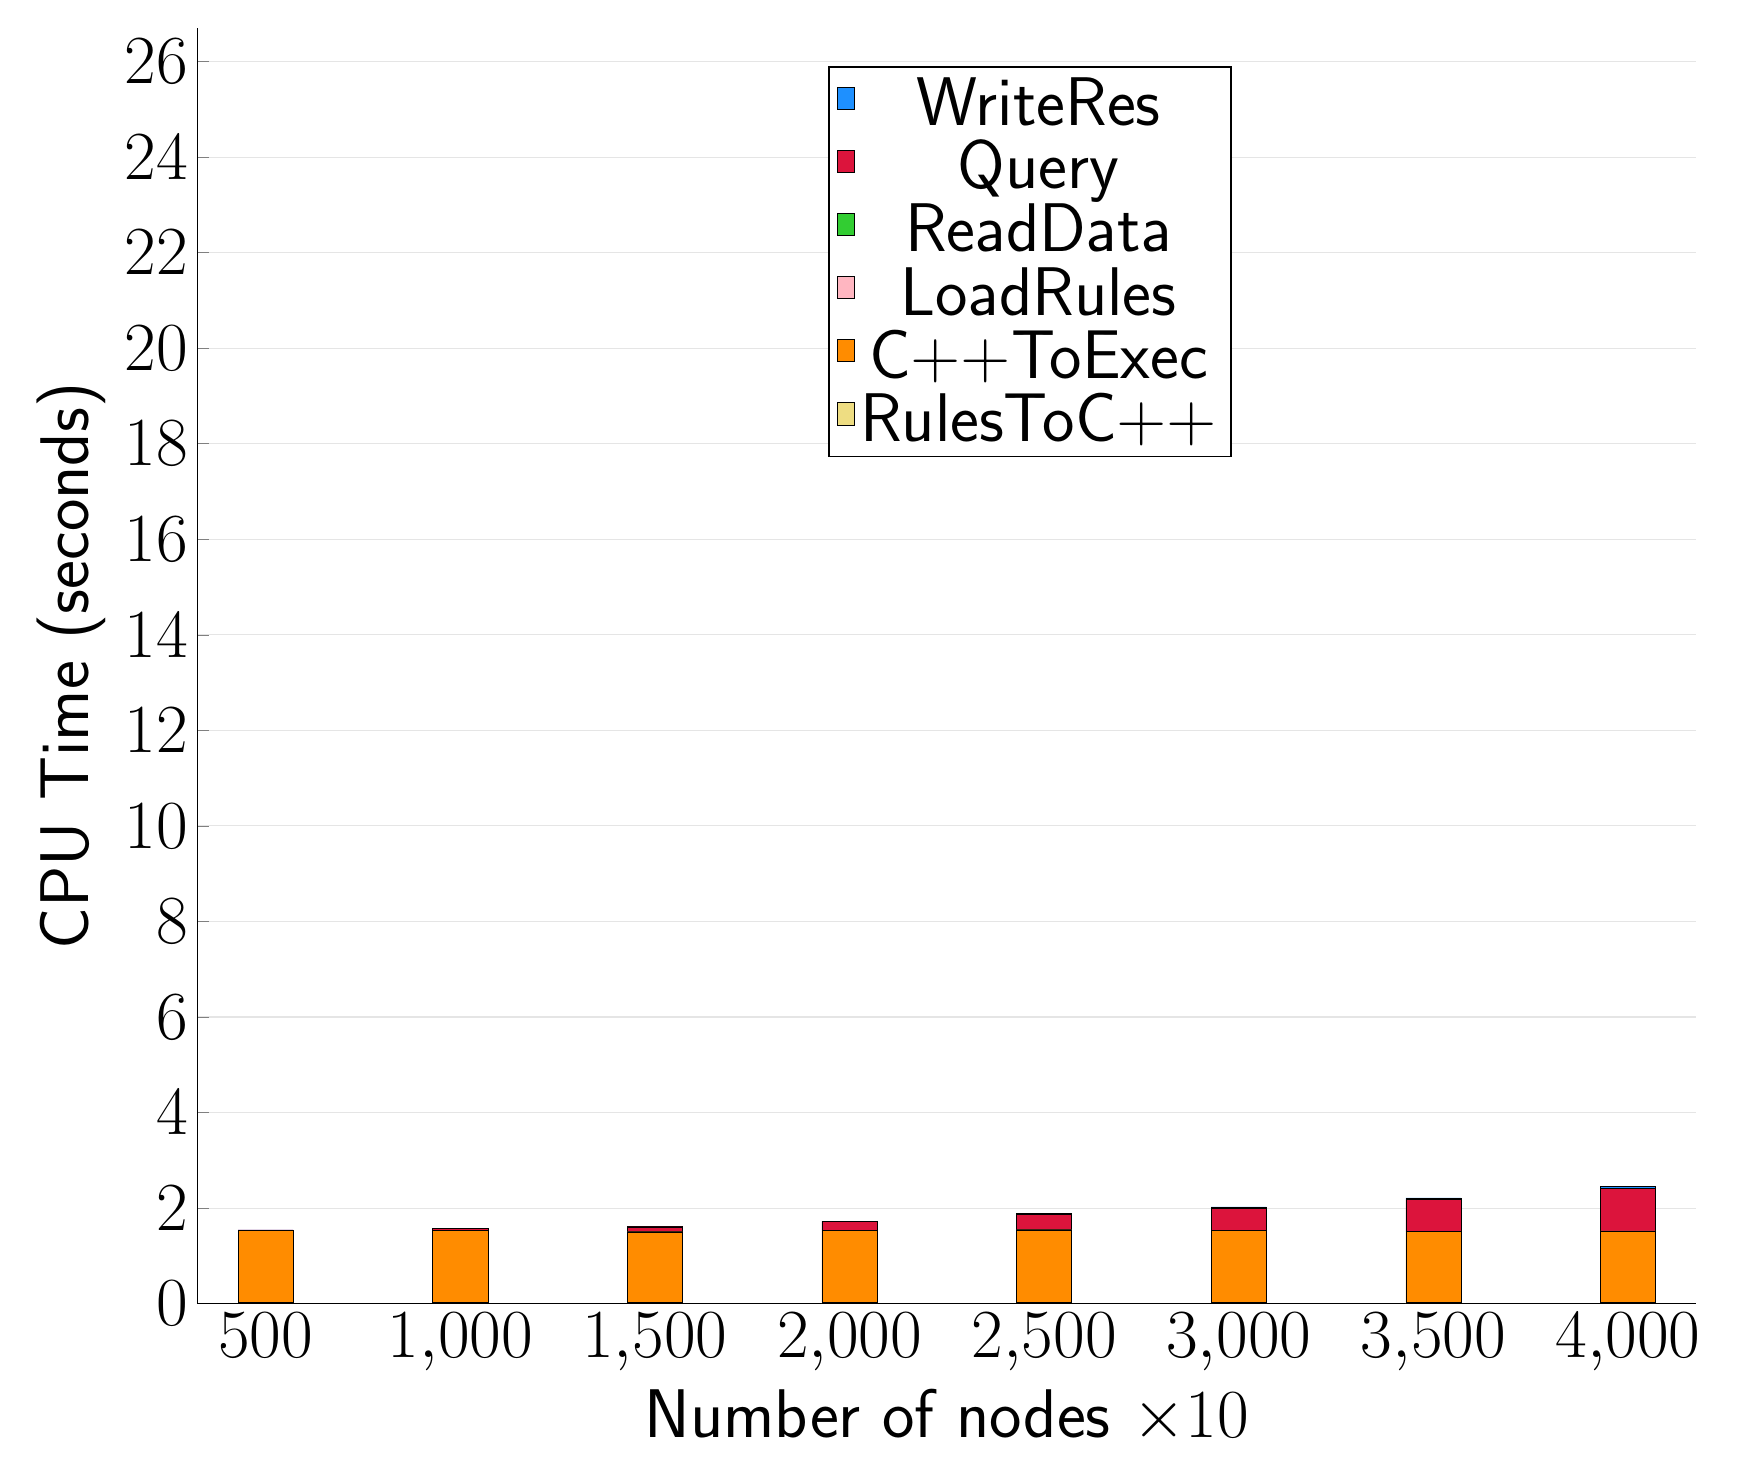
\begin{tikzpicture}
\begin{axis}[
   ybar stacked,
   width=1.7\textwidth,
   bar width=0.7cm,
   ymajorgrids, tick align=inside,
   major grid style={draw=gray!20},
   xtick=data,
   ymin=0, ymax=26.698890000000002,
   axis x line*=bottom,
   axis y line*=left,
   enlarge x limits=0.05,
   legend style={
       at={(0.69, 0.97)},
       anchor=north east,
       legend columns=1,
       font=\Huge,
   },
   ylabel={CPU Time (seconds)},
   xlabel={Number of nodes $\times 10$},
   label style={font=\Huge},
   tick label style={font=\Huge},
]
\addlegendimage{fill=DodgerBlue, draw=black, line width=0.2pt}
\addlegendentry{WriteRes}
\addlegendimage{fill=Crimson, draw=black, line width=0.2pt}
\addlegendentry{Query}
\addlegendimage{fill=LimeGreen, draw=black, line width=0.2pt}
\addlegendentry{ReadData}
\addlegendimage{fill=LightPink, draw=black, line width=0.2pt}
\addlegendentry{LoadRules}
\addlegendimage{fill=DarkOrange, draw=black, line width=0.2pt}
\addlegendentry{C++ToExec}
\addlegendimage{fill=LightGoldenrod, draw=black, line width=0.2pt}
\addlegendentry{RulesToC++}
\addplot +[fill=LightGoldenrod, draw=black, line width=0.2pt] coordinates {
(500, 0.030000000000000006)
(1000, 0.030000000000000006)
(1500, 0.030000000000000006)
(2000, 0.030000000000000006)
(2500, 0.030000000000000006)
(3000, 0.030000000000000006)
(3500, 0.030000000000000006)
(4000, 0.030000000000000006)
};
\addplot +[fill=DarkOrange, draw=black, line width=0.2pt] coordinates {
(500, 1.499)
(1000, 1.499)
(1500, 1.4700000000000002)
(2000, 1.498)
(2500, 1.5110000000000001)
(3000, 1.502)
(3500, 1.479)
(4000, 1.482)
};
\addplot +[fill=LightPink, draw=black, line width=0.2pt] coordinates {
(500, 9.549999999999999e-05)
(1000, 0.0001109)
(1500, 7.55e-05)
(2000, 9.52e-05)
(2500, 7.819999999999999e-05)
(3000, 0.00010410000000000001)
(3500, 0.0001227)
(4000, 0.000108)
};
\addplot +[fill=LimeGreen, draw=black, line width=0.2pt] coordinates {
(500, 0.0013733)
(1000, 0.0026395)
(1500, 0.0037284000000000006)
(2000, 0.0047845)
(2500, 0.0054067)
(3000, 0.0070896)
(3500, 0.0088945)
(4000, 0.0098764)
};
\addplot +[fill=Crimson, draw=black, line width=0.2pt] coordinates {
(500, 0.012786199999999998)
(1000, 0.044885800000000003)
(1500, 0.1024462)
(2000, 0.1844246)
(2500, 0.31751310000000005)
(3000, 0.46051449999999994)
(3500, 0.6629084000000001)
(4000, 0.8883324)
};
\addplot +[fill=DodgerBlue, draw=black, line width=0.2pt] coordinates {
(500, 0.0011163999999999998)
(1000, 0.0029163)
(1500, 0.0063707)
(2000, 0.0113031)
(2500, 0.017820500000000003)
(3000, 0.025337600000000005)
(3500, 0.034159100000000005)
(4000, 0.0449107)
};
\end{axis}
\end{tikzpicture}

\end{document}
